% Options for packages loaded elsewhere
\PassOptionsToPackage{unicode}{hyperref}
\PassOptionsToPackage{hyphens}{url}
\PassOptionsToPackage{dvipsnames,svgnames,x11names}{xcolor}
%
\documentclass[
  ignorenonframetext,
  aspectratio=169]{beamer}
\usepackage{pgfpages}
\setbeamertemplate{caption}[numbered]
\setbeamertemplate{caption label separator}{: }
\setbeamercolor{caption name}{fg=normal text.fg}
\beamertemplatenavigationsymbolsempty
% Prevent slide breaks in the middle of a paragraph
\widowpenalties 1 10000
\raggedbottom
\setbeamertemplate{part page}{
  \centering
  \begin{beamercolorbox}[sep=16pt,center]{part title}
    \usebeamerfont{part title}\insertpart\par
  \end{beamercolorbox}
}
\setbeamertemplate{section page}{
  \centering
  \begin{beamercolorbox}[sep=12pt,center]{part title}
    \usebeamerfont{section title}\insertsection\par
  \end{beamercolorbox}
}
\setbeamertemplate{subsection page}{
  \centering
  \begin{beamercolorbox}[sep=8pt,center]{part title}
    \usebeamerfont{subsection title}\insertsubsection\par
  \end{beamercolorbox}
}
\AtBeginPart{
  \frame{\partpage}
}
\AtBeginSection{
  \ifbibliography
  \else
    \frame{\sectionpage}
  \fi
}
\AtBeginSubsection{
  \frame{\subsectionpage}
}
\usepackage{amsmath,amssymb}
\usepackage{lmodern}
\usepackage{iftex}
\ifPDFTeX
  \usepackage[T1]{fontenc}
  \usepackage[utf8]{inputenc}
  \usepackage{textcomp} % provide euro and other symbols
\else % if luatex or xetex
  \usepackage{unicode-math}
  \defaultfontfeatures{Scale=MatchLowercase}
  \defaultfontfeatures[\rmfamily]{Ligatures=TeX,Scale=1}
\fi
\usetheme[]{CambridgeUS}
% Use upquote if available, for straight quotes in verbatim environments
\IfFileExists{upquote.sty}{\usepackage{upquote}}{}
\IfFileExists{microtype.sty}{% use microtype if available
  \usepackage[]{microtype}
  \UseMicrotypeSet[protrusion]{basicmath} % disable protrusion for tt fonts
}{}
\makeatletter
\@ifundefined{KOMAClassName}{% if non-KOMA class
  \IfFileExists{parskip.sty}{%
    \usepackage{parskip}
  }{% else
    \setlength{\parindent}{0pt}
    \setlength{\parskip}{6pt plus 2pt minus 1pt}}
}{% if KOMA class
  \KOMAoptions{parskip=half}}
\makeatother
\usepackage{xcolor}
\newif\ifbibliography
\usepackage{color}
\usepackage{fancyvrb}
\newcommand{\VerbBar}{|}
\newcommand{\VERB}{\Verb[commandchars=\\\{\}]}
\DefineVerbatimEnvironment{Highlighting}{Verbatim}{commandchars=\\\{\}}
% Add ',fontsize=\small' for more characters per line
\usepackage{framed}
\definecolor{shadecolor}{RGB}{248,248,248}
\newenvironment{Shaded}{\begin{snugshade}}{\end{snugshade}}
\newcommand{\AlertTok}[1]{\textcolor[rgb]{0.94,0.16,0.16}{#1}}
\newcommand{\AnnotationTok}[1]{\textcolor[rgb]{0.56,0.35,0.01}{\textbf{\textit{#1}}}}
\newcommand{\AttributeTok}[1]{\textcolor[rgb]{0.77,0.63,0.00}{#1}}
\newcommand{\BaseNTok}[1]{\textcolor[rgb]{0.00,0.00,0.81}{#1}}
\newcommand{\BuiltInTok}[1]{#1}
\newcommand{\CharTok}[1]{\textcolor[rgb]{0.31,0.60,0.02}{#1}}
\newcommand{\CommentTok}[1]{\textcolor[rgb]{0.56,0.35,0.01}{\textit{#1}}}
\newcommand{\CommentVarTok}[1]{\textcolor[rgb]{0.56,0.35,0.01}{\textbf{\textit{#1}}}}
\newcommand{\ConstantTok}[1]{\textcolor[rgb]{0.00,0.00,0.00}{#1}}
\newcommand{\ControlFlowTok}[1]{\textcolor[rgb]{0.13,0.29,0.53}{\textbf{#1}}}
\newcommand{\DataTypeTok}[1]{\textcolor[rgb]{0.13,0.29,0.53}{#1}}
\newcommand{\DecValTok}[1]{\textcolor[rgb]{0.00,0.00,0.81}{#1}}
\newcommand{\DocumentationTok}[1]{\textcolor[rgb]{0.56,0.35,0.01}{\textbf{\textit{#1}}}}
\newcommand{\ErrorTok}[1]{\textcolor[rgb]{0.64,0.00,0.00}{\textbf{#1}}}
\newcommand{\ExtensionTok}[1]{#1}
\newcommand{\FloatTok}[1]{\textcolor[rgb]{0.00,0.00,0.81}{#1}}
\newcommand{\FunctionTok}[1]{\textcolor[rgb]{0.00,0.00,0.00}{#1}}
\newcommand{\ImportTok}[1]{#1}
\newcommand{\InformationTok}[1]{\textcolor[rgb]{0.56,0.35,0.01}{\textbf{\textit{#1}}}}
\newcommand{\KeywordTok}[1]{\textcolor[rgb]{0.13,0.29,0.53}{\textbf{#1}}}
\newcommand{\NormalTok}[1]{#1}
\newcommand{\OperatorTok}[1]{\textcolor[rgb]{0.81,0.36,0.00}{\textbf{#1}}}
\newcommand{\OtherTok}[1]{\textcolor[rgb]{0.56,0.35,0.01}{#1}}
\newcommand{\PreprocessorTok}[1]{\textcolor[rgb]{0.56,0.35,0.01}{\textit{#1}}}
\newcommand{\RegionMarkerTok}[1]{#1}
\newcommand{\SpecialCharTok}[1]{\textcolor[rgb]{0.00,0.00,0.00}{#1}}
\newcommand{\SpecialStringTok}[1]{\textcolor[rgb]{0.31,0.60,0.02}{#1}}
\newcommand{\StringTok}[1]{\textcolor[rgb]{0.31,0.60,0.02}{#1}}
\newcommand{\VariableTok}[1]{\textcolor[rgb]{0.00,0.00,0.00}{#1}}
\newcommand{\VerbatimStringTok}[1]{\textcolor[rgb]{0.31,0.60,0.02}{#1}}
\newcommand{\WarningTok}[1]{\textcolor[rgb]{0.56,0.35,0.01}{\textbf{\textit{#1}}}}
\usepackage{longtable,booktabs,array}
\usepackage{calc} % for calculating minipage widths
\usepackage{caption}
% Make caption package work with longtable
\makeatletter
\def\fnum@table{\tablename~\thetable}
\makeatother
\setlength{\emergencystretch}{3em} % prevent overfull lines
\providecommand{\tightlist}{%
  \setlength{\itemsep}{0pt}\setlength{\parskip}{0pt}}
\setcounter{secnumdepth}{-\maxdimen} % remove section numbering
\ifLuaTeX
\usepackage[bidi=basic]{babel}
\else
\usepackage[bidi=default]{babel}
\fi
\babelprovide[main,import]{spanish}
% get rid of language-specific shorthands (see #6817):
\let\LanguageShortHands\languageshorthands
\def\languageshorthands#1{}

%\usepackage[spanish,es-nolists]{babel}
%%\usepackage[spanish]{babel}
%% change fontsize of R code
%%colorines
\usepackage{amsmath,color,array,booktabs,algorithm2e}
%\newcommand\blue[1]{\textcolor{blue}{#1}}
%\newcommand\red[1]{\textcolor{red}{#1}}

%% change fontsize of output
\let\oldverbatim\verbatim
\let\endoldverbatim\endverbatim
\renewenvironment{verbatim}{\tiny\oldverbatim}{\endoldverbatim}

%\usepackage[table,xcdraw]{xcolor}

\usepackage{makecell}
 \usepackage{booktabs}
 \usepackage{adjustbox}
 \usepackage{amsmath,color,array,booktabs,algorithm2e}
 \newcommand\blue[1]{\textcolor{blue}{#1}}
 \newcommand\red[1]{\textcolor{red}{#1}}
 \setbeamertemplate{navigation symbols}{}
 \setbeamertemplate{footline}[page number]
 \usepackage{mathdots}
\usepackage{yhmath}
\usepackage{mathdots}
\usepackage{MnSymbol}
\renewcommand{\contentsname}{Índice}
\renewcommand{\chaptername}{Parte}
\renewcommand{\sectionname}{Sección}
\ifLuaTeX
  \usepackage{selnolig}  % disable illegal ligatures
\fi
\IfFileExists{bookmark.sty}{\usepackage{bookmark}}{\usepackage{hyperref}}
\IfFileExists{xurl.sty}{\usepackage{xurl}}{} % add URL line breaks if available
\urlstyle{same} % disable monospaced font for URLs
\hypersetup{
  pdftitle={R básico},
  pdflang={es-ES},
  colorlinks=true,
  linkcolor={Maroon},
  filecolor={Maroon},
  citecolor={Blue},
  urlcolor={Blue},
  pdfcreator={LaTeX via pandoc}}

\title{R básico}
\author{}
\date{\vspace{-2.5em}10-2022}

\begin{document}
\frame{\titlepage}

\begin{frame}[allowframebreaks]
  \tableofcontents[hideallsubsections]
\end{frame}
\hypertarget{conociendo-r}{%
\section{Conociendo R}\label{conociendo-r}}

\begin{frame}{¿Qué es R?}
\protect\hypertarget{quuxe9-es-r}{}
\begin{figure}

\includegraphics[width=75px]{Imgs/Rlogo} \end{figure}

\begin{itemize}
\tightlist
\item
  Entorno de programación para el análisis estadístico y gráfico de
  datos
\item
  Software libre
\item
  Sintaxis sencilla e intuitiva
\item
  Enorme comunidad de usuarios (Comprehensive R Archive Network, CRAN)
\item
  ¿Aún tenéis dudas de por qué usarlo?
  \href{https://www.google.com/search?q=Why+use+R\&rlz=1C1CHBF_esES891ES891\&sxsrf=ALiCzsY4-woeo8PpPd0yw3j3b8guwp9zZQ\%3A1664188143209\&ei=734xY5C1DOaIur4PjI2XoAU\&ved=0ahUKEwjQ6PX4n7L6AhVmhM4BHYzGBVQQ4dUDCA4\&uact=5\&oq=Why+use+R\&gs_lcp=Cgdnd3Mtd2l6EAMyCggAEEcQ1gQQsAMyCggAEEcQ1gQQsAMyCggAEEcQ1gQQsAMyCggAEEcQ1gQQsAMyCggAEEcQ1gQQsAMyCggAEEcQ1gQQsAMyCggAEEcQ1gQQsAMyCggAEEcQ1gQQsAMyBwgAELADEENKBAhBGABKBAhGGABQAFgAYIMMaAFwAHgAgAEAiAEAkgEAmAEAyAEJwAEB\&sclient=gws-wiz}{Hay
  muchas opiniones en la web}
\end{itemize}
\end{frame}

\begin{frame}{¿Qué es RStudio?}
\protect\hypertarget{quuxe9-es-rstudio}{}
En este curso usaremos RStudio-desktop como interfaz gráfica de usuario
de R para todos los sistemas operativos

Es un entorno integrado para utilizar y programar con R

\begin{center}
\includegraphics[width=75px]{Imgs/RSLogo} \end{center}
\end{frame}

\begin{frame}[fragile]{Cómo instalar R}
\protect\hypertarget{cuxf3mo-instalar-r}{}
\textbf{Si sois de Windows o Mac}

\begin{enumerate}
\tightlist
\item
  Id a \href{http://cran.r-project.org/}{CRAN}
\item
  Pulsad sobre el enlace correspondiente a vuestro sistema operativo
\item
  Seguid las instrucciones de instalación correspondientes
\end{enumerate}

\textbf{Si trabajáis con Ubuntu o Debian}

\begin{enumerate}
\tightlist
\item
  Abrid la terminal, estando conectados a internet
\item
  Introducid lo siguiente: \texttt{sudo\ aptitude\ install\ r-base}
\end{enumerate}
\end{frame}

\begin{frame}[fragile]{Rstudio}
\protect\hypertarget{rstudio}{}
Un editor de \texttt{R} y muchas más cosas

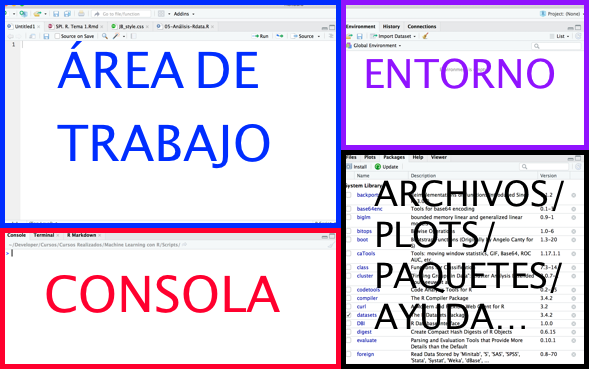
\includegraphics[width=0.7\linewidth]{Imgs/InterfazRStudio}
\end{frame}

\begin{frame}[fragile]{Cómo instalar RStudio}
\protect\hypertarget{cuxf3mo-instalar-rstudio}{}
\begin{enumerate}
\tightlist
\item
  \href{http://www.rstudio.com/products/rstudio/download/}{Obtener
  RStudio}
\item
  \textbf{Solo si utilizáis Linux}, ejecutad en una terminal la
  siguiente instrucción para completar la instalación:
  \texttt{sudo\ dpkg\ -i\ rstudio-\textless{}version\textgreater{}-i386.deb},
  donde \texttt{version} refiere a la versión concreta que se haya
  descargado
\end{enumerate}

\begin{center}
\includegraphics[width=75px]{Imgs/RSLogo} \end{center}
\end{frame}

\begin{frame}{Trabajando con RStudio}
\protect\hypertarget{trabajando-con-rstudio}{}
\begin{center}
\includegraphics[width=0.7\linewidth]{Imgs/easy_plus_tools} \end{center}
\end{frame}

\begin{frame}[fragile]{Cómo pedir ayuda}
\protect\hypertarget{cuxf3mo-pedir-ayuda}{}
\begin{itemize}
\tightlist
\item
  \texttt{help()}: obtener ayuda por consola
\item
  \texttt{??...}: obtener ayuda por consola
\item
  Pestaña \texttt{Help} de Rstudio
\item
  \href{https://www.rstudio.com/wp-content/uploads/2015/02/rmarkdown-cheatsheet.pdf}{Cheat
  Sheet de RStudio} y
  \href{https://www.google.com/search?q=Cheat+Sheet++RStudio\&rlz=1C1CHBF_esES891ES891\&sxsrf=ALiCzsYTamg5AX36RN8EhpV8lSO55ijfRw\%3A1664221782651\&ei=VgIyY5GzJ5nCa6rfovAP\&ved=0ahUKEwiRtrqhnbP6AhUZ4RoKHaqvCP4Q4dUDCA4\&uact=5\&oq=Cheat+Sheet++RStudio\&gs_lcp=Cgdnd3Mtd2l6EAMyCAgAEB4QBxATMggIABAeEAUQEzIICAAQHhAFEBMyCAgAEB4QBRATMggIABAeEAUQEzIICAAQHhAFEBMyCAgAEB4QBRATMggIABAeEAgQEzIICAAQHhAIEBMyCAgAEB4QCBATOgoIABBHENYEELADOggIABAeEAgQB0oECEEYAEoECEYYAFCmCljnC2DOEWgBcAF4AIABaogBzQGSAQMxLjGYAQCgAQHIAQjAAQE\&sclient=gws-wiz}{más}
\item
  Buscad por la red (stackoverflow, R project\ldots)
\end{itemize}
\end{frame}

\begin{frame}[fragile]{Paquetes: cómo instalarlos y cargarlos}
\protect\hypertarget{paquetes-cuxf3mo-instalarlos-y-cargarlos}{}
\blue{Paquete/librería}. Un \textbf{package} es una librería de
funciones y datos que que pueden venir o no instaladas en la carga de R
básico.

\begin{itemize}
\tightlist
\item
  \texttt{install.packages("nombre\_paquete",\ dep\ =\ TRUE)}: instala o
  actualiza un paquete de R
\item
  \texttt{library(nombre\_del\_paquete)}: carga un paquete ya instalado
\end{itemize}
\end{frame}

\hypertarget{operaciones-buxe1sicas}{%
\section{Operaciones básicas}\label{operaciones-buxe1sicas}}

\begin{frame}[fragile]{Operaciones}
\protect\hypertarget{operaciones}{}
\begin{longtable}[]{@{}ll@{}}
\toprule()
Código & Operación \\
\midrule()
\endhead
\texttt{+} & Suma \\
\texttt{-} & Resta \\
\texttt{*} & Multiplicación \\
\texttt{/} & División \\
\texttt{\^{}} & Potencia \\
\texttt{\%/\%} & Cociente entero \\
\texttt{\%\%} & Resto de división entera \\
\bottomrule()
\end{longtable}
\end{frame}

\begin{frame}[fragile]{Calculadora básica - Operaciones}
\protect\hypertarget{calculadora-buxe1sica---operaciones}{}
\begin{longtable}[]{@{}ll@{}}
\toprule()
Código & Significado \\
\midrule()
\endhead
\texttt{pi} & {[}\(\pi\){]} \\
\texttt{Inf} &
\href{https://es.wikipedia.org/wiki/Infinito}{\(\infty\)} \\
\texttt{NaN} & Indeterminación (Not a Number) \\
\texttt{NA} & Valor desconocido (Not Available) \\
\bottomrule()
\end{longtable}
\end{frame}

\begin{frame}[fragile]{Calculadora básica - Operaciones}
\protect\hypertarget{calculadora-buxe1sica---operaciones-1}{}
\begin{Shaded}
\begin{Highlighting}[]
\DecValTok{2}\SpecialCharTok{+}\DecValTok{2}
\end{Highlighting}
\end{Shaded}

\begin{verbatim}
[1] 4
\end{verbatim}

\begin{Shaded}
\begin{Highlighting}[]
\DecValTok{77}\SpecialCharTok{\%/\%}\DecValTok{5}
\end{Highlighting}
\end{Shaded}

\begin{verbatim}
[1] 15
\end{verbatim}

\begin{Shaded}
\begin{Highlighting}[]
\DecValTok{77}\SpecialCharTok{\%\%}\DecValTok{5}
\end{Highlighting}
\end{Shaded}

\begin{verbatim}
[1] 2
\end{verbatim}
\end{frame}

\begin{frame}[fragile]{Funciones básicas}
\protect\hypertarget{funciones-buxe1sicas}{}
\begin{longtable}[]{@{}ll@{}}
\toprule()
Código & Función \\
\midrule()
\endhead
\texttt{sqrt(x)} & \(\sqrt{x}\) \\
\texttt{exp(x)} & \(e^x\) \\
\texttt{log(x)} & \(\ln(x)\) \\
\texttt{log10(x)} & \(\log_{10}(x)\) \\
\texttt{log(x,a)} & \(\log_a(x)\) \\
\texttt{abs(x)} & \(\begin{vmatrix}x\end{vmatrix}\) \\
\bottomrule()
\end{longtable}
\end{frame}

\begin{frame}[fragile]{Funciones básicas}
\protect\hypertarget{funciones-buxe1sicas-1}{}
\begin{Shaded}
\begin{Highlighting}[]
\FunctionTok{sqrt}\NormalTok{(}\DecValTok{9}\NormalTok{)}
\end{Highlighting}
\end{Shaded}

\begin{verbatim}
[1] 3
\end{verbatim}

\begin{Shaded}
\begin{Highlighting}[]
\FunctionTok{log}\NormalTok{(}\FunctionTok{exp}\NormalTok{(}\DecValTok{1}\NormalTok{))}
\end{Highlighting}
\end{Shaded}

\begin{verbatim}
[1] 1
\end{verbatim}

\begin{Shaded}
\begin{Highlighting}[]
\FunctionTok{log}\NormalTok{(}\DecValTok{1000}\NormalTok{,}\DecValTok{10}\NormalTok{)}
\end{Highlighting}
\end{Shaded}

\begin{verbatim}
[1] 3
\end{verbatim}

\begin{Shaded}
\begin{Highlighting}[]
\FunctionTok{log10}\NormalTok{(}\DecValTok{1000}\NormalTok{)}
\end{Highlighting}
\end{Shaded}

\begin{verbatim}
[1] 3
\end{verbatim}
\end{frame}

\begin{frame}[fragile]{Combinatoria básica}
\protect\hypertarget{combinatoria-buxe1sica}{}
\begin{longtable}[]{@{}ll@{}}
\toprule()
Código & Operación \\
\midrule()
\endhead
\texttt{factorial(x)} &
\href{https://es.wikipedia.org/wiki/Factorial}{x!} \\
\texttt{choose(n,m)} & \(\begin{pmatrix}n\\ m\end{pmatrix}\) \\
\bottomrule()
\end{longtable}

\vspace{0.2cm}

\begin{itemize}
\item
  \blue{Número factorial.}

  Se define como número factorial de un número entero positivo \(n\)
  como \(n!=n\cdot(n-1)\cdots 2\cdot 1\)
\item
  \href{https://es.wikipedia.org/wiki/Coeficiente_binomial}{Coeficiente
  binomial}. Se define el coeficiente binomial de \(n\) sobre \(m\) como
  \[\begin{pmatrix}n\\ m\end{pmatrix}=\frac{n!}{m!(n-m)!}\]
\end{itemize}
\end{frame}

\begin{frame}[fragile]{Calculadora básica - Combinatoria}
\protect\hypertarget{calculadora-buxe1sica---combinatoria}{}
\begin{Shaded}
\begin{Highlighting}[]
\FunctionTok{factorial}\NormalTok{(}\DecValTok{5}\NormalTok{)}
\end{Highlighting}
\end{Shaded}

\begin{verbatim}
[1] 120
\end{verbatim}

\begin{Shaded}
\begin{Highlighting}[]
\FunctionTok{choose}\NormalTok{(}\DecValTok{4}\NormalTok{,}\DecValTok{2}\NormalTok{)}
\end{Highlighting}
\end{Shaded}

\begin{verbatim}
[1] 6
\end{verbatim}

\begin{Shaded}
\begin{Highlighting}[]
\FunctionTok{factorial}\NormalTok{(}\DecValTok{6}\NormalTok{)}
\end{Highlighting}
\end{Shaded}

\begin{verbatim}
[1] 720
\end{verbatim}

\begin{Shaded}
\begin{Highlighting}[]
\FunctionTok{factorial}\NormalTok{(}\DecValTok{5}\NormalTok{)}\SpecialCharTok{*}\DecValTok{6}
\end{Highlighting}
\end{Shaded}

\begin{verbatim}
[1] 720
\end{verbatim}
\end{frame}

\begin{frame}[fragile]{Trigonometría en radianes}
\protect\hypertarget{trigonometruxeda-en-radianes}{}
\begin{longtable}[]{@{}ll@{}}
\toprule()
Código & Función \\
\midrule()
\endhead
\texttt{sin(x)} & \(\sin(x)\) \\
\texttt{cos(x)} & \(\cos(x)\) \\
\texttt{tan(x)} & \(\tan(x)\) \\
\texttt{asin(x)} & \(\arcsin(x)\) \\
\texttt{acos(x)} & \(\arccos(x)\) \\
\texttt{atan(x)} & \(\arctan(x)\) \\
\bottomrule()
\end{longtable}
\end{frame}

\begin{frame}[fragile]{Trigonometría en radianes}
\protect\hypertarget{trigonometruxeda-en-radianes-1}{}
\begin{Shaded}
\begin{Highlighting}[]
\FunctionTok{sin}\NormalTok{(pi}\SpecialCharTok{/}\DecValTok{2}\NormalTok{)}
\end{Highlighting}
\end{Shaded}

\begin{verbatim}
[1] 1
\end{verbatim}

\begin{Shaded}
\begin{Highlighting}[]
\FunctionTok{cos}\NormalTok{(pi)}
\end{Highlighting}
\end{Shaded}

\begin{verbatim}
[1] -1
\end{verbatim}

\begin{Shaded}
\begin{Highlighting}[]
\FunctionTok{tan}\NormalTok{(}\DecValTok{0}\NormalTok{)}
\end{Highlighting}
\end{Shaded}

\begin{verbatim}
[1] 0
\end{verbatim}
\end{frame}

\begin{frame}[fragile]{Un ejemplo de gráficos}
\protect\hypertarget{un-ejemplo-de-gruxe1ficos}{}
\begin{Shaded}
\begin{Highlighting}[]
\NormalTok{x }\OtherTok{=} \FunctionTok{seq}\NormalTok{(}\DecValTok{0}\NormalTok{,}\DecValTok{2}\SpecialCharTok{*}\NormalTok{pi,}\FloatTok{0.1}\NormalTok{)}
\FunctionTok{plot}\NormalTok{(x,}\FunctionTok{sin}\NormalTok{(x),}\AttributeTok{type=}\StringTok{"l"}\NormalTok{,}\AttributeTok{col=}\StringTok{"blue"}\NormalTok{,}\AttributeTok{lwd=}\DecValTok{3}\NormalTok{, }
     \AttributeTok{xlab=}\FunctionTok{expression}\NormalTok{(x), }\AttributeTok{ylab=}\StringTok{""}\NormalTok{,}
     \AttributeTok{xlim=}\FunctionTok{c}\NormalTok{(}\DecValTok{0}\NormalTok{,}\DecValTok{4}\NormalTok{),}\AttributeTok{cex=}\FloatTok{0.5}\NormalTok{)}
\FunctionTok{curve}\NormalTok{(}\FunctionTok{cos}\NormalTok{(x),}\AttributeTok{col=}\StringTok{"red"}\NormalTok{,}\AttributeTok{add=}\ConstantTok{TRUE}\NormalTok{)}
\FunctionTok{lines}\NormalTok{(x, }\FunctionTok{tan}\NormalTok{(x}\SpecialCharTok{/}\DecValTok{2}\NormalTok{), }\AttributeTok{col=}\StringTok{"purple"}\NormalTok{,}\AttributeTok{lwd=}\DecValTok{3}\NormalTok{)}
\FunctionTok{legend}\NormalTok{(}\StringTok{"bottomleft"}\NormalTok{,}
       \AttributeTok{col=}\FunctionTok{c}\NormalTok{(}\StringTok{"blue"}\NormalTok{,}\StringTok{"green"}\NormalTok{,}\StringTok{"purple"}\NormalTok{),}
       \AttributeTok{legend=}\FunctionTok{c}\NormalTok{(}\StringTok{"Seno"}\NormalTok{,}\StringTok{"Coseno"}\NormalTok{, }\StringTok{"Tangente"}\NormalTok{),}
       \AttributeTok{lwd=}\DecValTok{3}\NormalTok{, }\AttributeTok{bty=}\StringTok{"l"}\NormalTok{,}\AttributeTok{cex=}\FloatTok{0.8}\NormalTok{)}
\end{Highlighting}
\end{Shaded}
\end{frame}

\begin{frame}{Un ejemplo de gráficos}
\protect\hypertarget{un-ejemplo-de-gruxe1ficos-1}{}
\ldots{} en tamaño normal

\begin{center}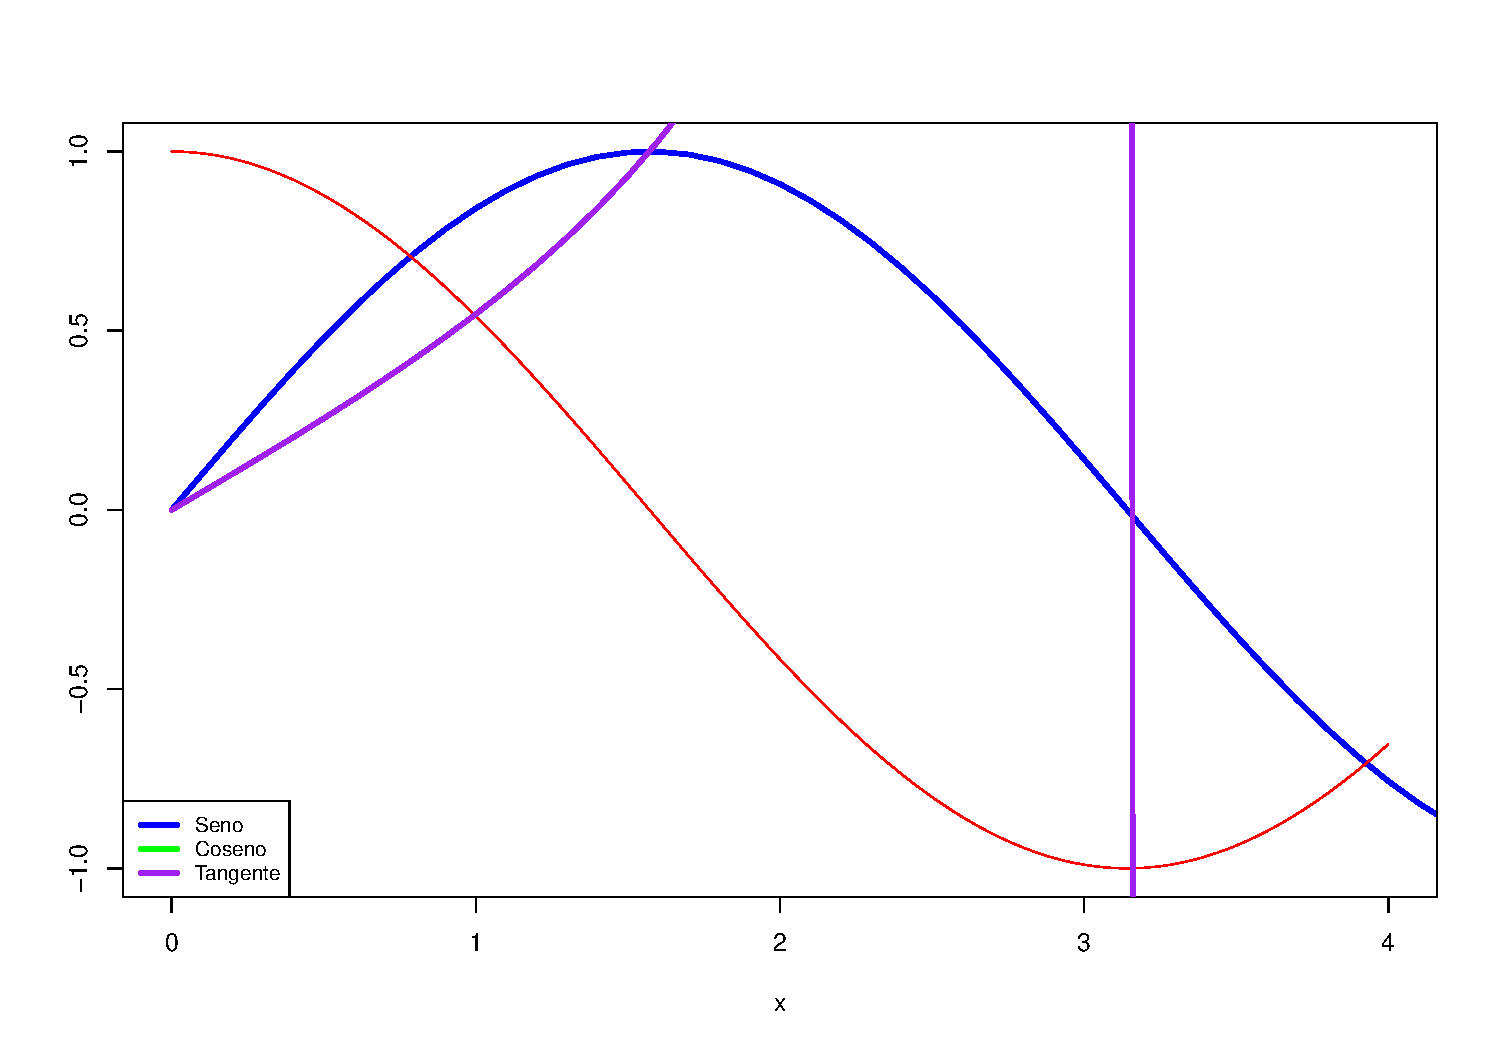
\includegraphics[width=0.6\linewidth]{Hora1_files/figure-beamer/plot2_tema1-1} \end{center}
\end{frame}

\begin{frame}[fragile]{Números en coma flotante}
\protect\hypertarget{nuxfameros-en-coma-flotante}{}
\begin{longtable}[]{@{}
  >{\raggedright\arraybackslash}p{(\columnwidth - 2\tabcolsep) * \real{0.2593}}
  >{\raggedright\arraybackslash}p{(\columnwidth - 2\tabcolsep) * \real{0.7407}}@{}}
\toprule()
\begin{minipage}[b]{\linewidth}\raggedright
Código
\end{minipage} & \begin{minipage}[b]{\linewidth}\raggedright
Función
\end{minipage} \\
\midrule()
\endhead
\texttt{print(x,n)} & Muestra las \(n\) cifras significativa del número
\(x\) \\
\texttt{round(x,n)} & Redondea a \(n\) cifras significativas un
resultado o vector numérico \(x\) \\
\texttt{floor(x)} & \(\lfloor x\rfloor\), parte entera por defecto de
\(x\) \\
\texttt{ceiling(x)} & \(\lceil x\rceil\), parte entera por exceso de
\(x\) \\
\texttt{trunc(x)} & Parte entera de \(x\), eliminando la parte
decimal \\
\bottomrule()
\end{longtable}
\end{frame}

\begin{frame}[fragile]{Números en coma flotante}
\protect\hypertarget{nuxfameros-en-coma-flotante-1}{}
\begin{Shaded}
\begin{Highlighting}[]
\FunctionTok{print}\NormalTok{(pi,}\DecValTok{5}\NormalTok{)}
\end{Highlighting}
\end{Shaded}

\begin{verbatim}
[1] 3.1416
\end{verbatim}

\begin{Shaded}
\begin{Highlighting}[]
\FunctionTok{round}\NormalTok{(pi,}\DecValTok{5}\NormalTok{)}
\end{Highlighting}
\end{Shaded}

\begin{verbatim}
[1] 3.14159
\end{verbatim}

\begin{Shaded}
\begin{Highlighting}[]
\FunctionTok{floor}\NormalTok{(pi)}
\end{Highlighting}
\end{Shaded}

\begin{verbatim}
[1] 3
\end{verbatim}

\begin{Shaded}
\begin{Highlighting}[]
\FunctionTok{ceiling}\NormalTok{(pi)}
\end{Highlighting}
\end{Shaded}

\begin{verbatim}
[1] 4
\end{verbatim}
\end{frame}

\begin{frame}[fragile]{Variables y funciones}
\protect\hypertarget{variables-y-funciones}{}
\begin{itemize}
\tightlist
\item
  \texttt{nombre\_variable\ =\ valor}: define una variable con dicho
  valor
\item
  \texttt{nombre\_función\ =\ function(variable)\{función\}}: define una
  función
\end{itemize}

\begin{Shaded}
\begin{Highlighting}[]
\NormalTok{a}\OtherTok{=} \DecValTok{8}
\NormalTok{cubo }\OtherTok{=} \ControlFlowTok{function}\NormalTok{(x)\{x}\SpecialCharTok{\^{}}\DecValTok{3}\NormalTok{\}}
\FunctionTok{cubo}\NormalTok{(}\AttributeTok{x=}\NormalTok{a)}
\end{Highlighting}
\end{Shaded}

\begin{verbatim}
[1] 512
\end{verbatim}

\begin{Shaded}
\begin{Highlighting}[]
\NormalTok{raiz\_cúbica }\OtherTok{=} \ControlFlowTok{function}\NormalTok{(x)\{x}\SpecialCharTok{\^{}}\NormalTok{(}\DecValTok{1}\SpecialCharTok{/}\DecValTok{3}\NormalTok{)\}}
\NormalTok{raiz\_cúbica(a)}
\end{Highlighting}
\end{Shaded}

\begin{verbatim}
[1] 2
\end{verbatim}

\begin{Shaded}
\begin{Highlighting}[]
\NormalTok{raiz\_cúbica(}\FunctionTok{cubo}\NormalTok{(}\AttributeTok{x=}\NormalTok{a))}
\end{Highlighting}
\end{Shaded}

\begin{verbatim}
[1] 8
\end{verbatim}
\end{frame}

\hypertarget{r-markdown}{%
\section{R Markdown}\label{r-markdown}}

\begin{frame}{Introducción}
\protect\hypertarget{introducciuxf3n}{}
\blue{R Markdown.} Es un tipo de fichero-programa en el cual podemos
intercalar sin problema alguno texto, código y fórmulas matemáticas.

Para la mayor parte de las necesidades de este curso, en lo referente a
la creación y composición de este tipo de ficheros, el documento
\emph{\href{https://en.support.wordpress.com/markdown-quick-reference/}{Markdown
Quick Reference} } y la
\href{http://shiny.rstudio.com/images/rm-cheatsheet.pdf.zip.}{chuleta}
de R Markdown deberían ser suficientes.

Sin embargo, a lo largo de este curso iremos ampliando estos contenidos
en algunos temas cuando lo creamos necesario.

Nosotros, en este tema, veremos cómo controlar el comportamiento de los
bloques de código (\blue{chunks}) al compilar el fichero R Markdown y
cómo escribir fórmulas matemáticas bien formateadas.
\end{frame}

\begin{frame}{Fórmulas matemáticas}
\protect\hypertarget{fuxf3rmulas-matemuxe1ticas}{}
Para escribir fórmulas matemáticas bien formateadas utilizaremos la
sintaxis \LaTeX

\begin{itemize}
\tightlist
\item
  Para tener ecuaciones o fórmulas en el mismo párrafo, escribimos
  nuestro código entre dos símbolos de dólar: código
\item
  Si queremos tener ecuaciones o fórmulas centradas en un párrafo
  aparte, escribimos nuestro código entre dos dobles símbolos de dólar:
  código
\end{itemize}

\red{¡Cuidado!} Al escribir una fórmula de la forma indicada
anteriormente o simplemente texto en R Markdown, los espacios en blanco
son completamente ignorados. RStudio solamente añade los espacios en
blanco a partir del significado lógico de sus elementos.
\end{frame}

\begin{frame}{Símbolos}
\protect\hypertarget{suxedmbolos}{}
Hay muchísimos símbolos matemáticos que puedes escribirse con la
sintaxis \LaTeX. En el ejemplo anterior ya os hemos mostrado unos pocos.
En este tema, nosotros solo veremos los más utilizados.

Para quien quiera ir más allá, aquí os dejamos un
\href{http://www.ptep-online.com/ctan/symbols.pdf}{documento muy útil}
con gran cantidad de símbolos de \LaTeX.
\end{frame}

\begin{frame}[fragile]{Símbolos matemáticos - Básico}
\protect\hypertarget{suxedmbolos-matemuxe1ticos---buxe1sico}{}
\begin{longtable}[]{@{}lll@{}}
\toprule()
Significado & Código & Resultado \\
\midrule()
\endhead
Suma & \texttt{+} & \(+\) \\
Resta & \texttt{-} & \(-\) \\
Producto & \texttt{\textbackslash{}cdot} & \(\cdot\) \\
Producto & \texttt{\textbackslash{}times} & \(\times\) \\
División & \texttt{\textbackslash{}div} & \(\div\) \\
Potencia & \texttt{a\^{}\{x\}} & \(a^{x}\) \\
Subíndice & \texttt{a\_\{i\}} & \(a_{i}\) \\
\bottomrule()
\end{longtable}
\end{frame}

\begin{frame}[fragile]{Símbolos matemáticos - Básico}
\protect\hypertarget{suxedmbolos-matemuxe1ticos---buxe1sico-1}{}
\begin{longtable}[]{@{}lll@{}}
\toprule()
Significado & Código & Resultado \\
\midrule()
\endhead
Fracción & \texttt{\textbackslash{}frac\{a\}\{b\}} & \(\frac{a}{b}\) \\
Más menos & \texttt{\textbackslash{}pm} & \(\pm\) \\
Raíz n-ésima & \texttt{\textbackslash{}sqrt{[}n{]}\{x\}} &
\(\sqrt[n]{x}\) \\
Unión & \texttt{cup} & \(\cup\) \\
Intersección & \texttt{\textbackslash{}cap} & \(\cap\) \\
OR lógico & \texttt{\textbackslash{}vee} & \(\vee\) \\
AND lógico & \texttt{\textbackslash{}wedge} & \(\wedge\) \\
\bottomrule()
\end{longtable}
\end{frame}

\begin{frame}[fragile]{Símbolos matemáticos - Relaciones}
\protect\hypertarget{suxedmbolos-matemuxe1ticos---relaciones}{}
\begin{longtable}[]{@{}lll@{}}
\toprule()
Significado & Código & Resultado \\
\midrule()
\endhead
Igual & \texttt{=} & \(=\) \\
Aproximado & \texttt{\textbackslash{}approx} & \(\approx\) \\
No igual & \texttt{\textbackslash{}ne} & \(\ne\) \\
Mayor que & \texttt{\textgreater{}} & \(>\) \\
Menor que & \texttt{\textless{}} & \(<\) \\
Mayor o igual que & \texttt{\textbackslash{}geq} & \(\geq\) \\
Menor o igual que & \texttt{\textbackslash{}leq} & \(\leq\) \\
\bottomrule()
\end{longtable}
\end{frame}

\begin{frame}[fragile]{Símbolos matemáticos - Operadores}
\protect\hypertarget{suxedmbolos-matemuxe1ticos---operadores}{}
\begin{longtable}[]{@{}lll@{}}
\toprule()
Significado & Código & Resultado \\
\midrule()
\endhead
Sumatorio & \texttt{\textbackslash{}sum\_\{i=0\}\^{}\{n\}} &
\(\sum_{i=0}^{n}\) \\
Productorio & \texttt{\textbackslash{}prod\_\{i=0\}\^{}\{n\}} &
\(\prod_{i=0}^{n}\) \\
Integral & \texttt{\textbackslash{}int\_\{a\}\^{}\{b\}} &
\(\int_{a}^{b}\) \\
Unión (grande) & \texttt{\textbackslash{}bigcup} & \(\bigcup\) \\
Intersección (grande) & \texttt{\textbackslash{}bigcap} & \(\bigcap\) \\
OR lógico (grande) & \texttt{\textbackslash{}bigvee} & \(\bigvee\) \\
AND lógico (grande) & \texttt{\textbackslash{}bigwedge} &
\(\bigwedge\) \\
\bottomrule()
\end{longtable}
\end{frame}

\begin{frame}[fragile]{Símbolos matemáticos - Delimitadores}
\protect\hypertarget{suxedmbolos-matemuxe1ticos---delimitadores}{}
\begin{longtable}[]{@{}lll@{}}
\toprule()
Significado & Código & Resultado \\
\midrule()
\endhead
Paréntesis & \texttt{()} & \((\ )\) \\
Corchetes & \texttt{{[}{]}} & \([\ ]\) \\
Llaves & \texttt{\textbackslash{}\{\ \textbackslash{}\}} & \(\{\ \}\) \\
Diamante & \texttt{\textbackslash{}langle\ \textbackslash{}rangle} &
\(\langle\ \rangle\) \\
Parte entera por defecto &
\texttt{\textbackslash{}lfloor\ \textbackslash{}rfloor} &
\(\lfloor\  \rfloor\) \\
Parte entera por exceso &
\texttt{\textbackslash{}lceil\ \textbackslash{}rceil} &
\(\lceil\ \rceil\) \\
Espacio en blanco & \texttt{hola\textbackslash{}\ caracola} &
\(hola\ caracola\) \\
\bottomrule()
\end{longtable}
\end{frame}

\begin{frame}[fragile]{Símbolos matemáticos - Letras griegas}
\protect\hypertarget{suxedmbolos-matemuxe1ticos---letras-griegas}{}
\begin{longtable}[]{@{}lll@{}}
\toprule()
Significado & Código & Resultado \\
\midrule()
\endhead
Alpha & \texttt{\textbackslash{}alpha} & \(\alpha\) \\
Beta & \texttt{\textbackslash{}beta} & \(\beta\) \\
Gamma & \texttt{\textbackslash{}gamma\ \textbackslash{}Gamma} &
\(\gamma\  \Gamma\) \\
Delta & \texttt{\textbackslash{}delta\ \textbackslash{}Delta} &
\(\delta\  \Delta\) \\
Epsilon & \texttt{\textbackslash{}epsilon} & \(\epsilon\) \\
Epsilon & \texttt{\textbackslash{}varepsilon} & \(\varepsilon\) \\
Zeta & \texttt{\textbackslash{}zeta} & \(\zeta\) \\
\bottomrule()
\end{longtable}
\end{frame}

\begin{frame}[fragile]{Símbolos matemáticos - Letras griegas}
\protect\hypertarget{suxedmbolos-matemuxe1ticos---letras-griegas-1}{}
\begin{longtable}[]{@{}lll@{}}
\toprule()
Significado & Código & Resultado \\
\midrule()
\endhead
Eta & \texttt{\textbackslash{}eta} & \(\eta\) \\
Theta & \texttt{\textbackslash{}theta\ \textbackslash{}Theta} &
\(\theta\ \Theta\) \\
Kappa & \texttt{\textbackslash{}kappa} & \(\kappa\) \\
Lambda & \texttt{\textbackslash{}lambda\ \textbackslash{}Lambda} &
\(\lambda\  \Lambda\) \\
Mu & \texttt{\textbackslash{}mu} & \(\mu\) \\
Nu & \texttt{\textbackslash{}nu} & \(\nu\) \\
Xi & \texttt{\textbackslash{}xi\ \textbackslash{}Xi} & \(\xi\ \Xi\) \\
\bottomrule()
\end{longtable}
\end{frame}

\begin{frame}[fragile]{Símbolos matemáticos - Letras griegas}
\protect\hypertarget{suxedmbolos-matemuxe1ticos---letras-griegas-2}{}
\begin{longtable}[]{@{}lll@{}}
\toprule()
Significado & Código & Resultado \\
\midrule()
\endhead
Pi & \texttt{\textbackslash{}pi\ \textbackslash{}Pi} & \(\pi\ \Pi\) \\
Rho & \texttt{\textbackslash{}rho} & \(\rho\) \\
Sigma & \texttt{\textbackslash{}sigma\ \textbackslash{}Sigma} &
\(\sigma\ \Sigma\) \\
Tau & \texttt{\textbackslash{}tau} & \(\tau\) \\
Upsilon & \texttt{\textbackslash{}upsilon\ \textbackslash{}Upsilon} &
\(\upsilon\ \Upsilon\) \\
Phi & \texttt{\textbackslash{}phi\ \textbackslash{}Phi} &
\(\phi\ \Phi\) \\
Phi & \texttt{\textbackslash{}varphi} & \(\varphi\) \\
\bottomrule()
\end{longtable}
\end{frame}

\begin{frame}[fragile]{Símbolos matemáticos - Letras griegas}
\protect\hypertarget{suxedmbolos-matemuxe1ticos---letras-griegas-3}{}
\begin{longtable}[]{@{}lll@{}}
\toprule()
Significado & Código & Resultado \\
\midrule()
\endhead
Chi & \texttt{\textbackslash{}chi} & \(\chi\) \\
Psi & \texttt{\textbackslash{}psi\ \textbackslash{}Psi} &
\(\psi\ \Psi\) \\
Omega & \texttt{\textbackslash{}omega\ \textbackslash{}Omega} &
\(\omega\ \Omega\) \\
\bottomrule()
\end{longtable}
\end{frame}

\begin{frame}[fragile]{Símbolos matemáticos - Acentos matemáticos}
\protect\hypertarget{suxedmbolos-matemuxe1ticos---acentos-matemuxe1ticos}{}
\begin{longtable}[]{@{}lll@{}}
\toprule()
Significado & Código & Resultado \\
\midrule()
\endhead
Gorrito & \texttt{\textbackslash{}hat\{x\}} & \(\hat{x}\) \\
Barra & \texttt{\textbackslash{}bar\{x\}} & \(\bar{x}\) \\
Punto 1 & \texttt{\textbackslash{}dot\{x\}} & \(\dot{x}\) \\
Punto 2 & \texttt{\textbackslash{}ddot\{x\}} & \(\ddot{x}\) \\
Punto 3 & \texttt{\textbackslash{}dddot\{x\}} & \(\dddot{x}\) \\
Tilde & \texttt{\textbackslash{}tilde\{x\}} & \(\tilde{x}\) \\
Vector & \texttt{\textbackslash{}vec\{x\}} & \(\vec{x}\) \\
\bottomrule()
\end{longtable}
\end{frame}

\begin{frame}[fragile]{Símbolos matemáticos - Acentos expansibles}
\protect\hypertarget{suxedmbolos-matemuxe1ticos---acentos-expansibles}{}
\begin{longtable}[]{@{}lll@{}}
\toprule()
Significado & Código & Resultado \\
\midrule()
\endhead
Gorrito & \texttt{\textbackslash{}widehat\{xyz\}} & \(\widehat{xyz}\) \\
Barra & \texttt{\textbackslash{}overline\{xyz\}} & \(\overline{xyz}\) \\
Subrallado & \texttt{\textbackslash{}underline\{xyz\}} &
\(\underline{xyz}\) \\
Llave superior & \texttt{\textbackslash{}overbrace\{xyz\}} &
\(\overbrace{xyz}\) \\
Llave inferior & \texttt{\textbackslash{}underbrace\{xyz\}} &
\(\underbrace{xyz}\) \\
Tilde & \texttt{\textbackslash{}widetilde\{xyz\}} &
\(\widetilde{xyz}\) \\
Vector & \texttt{\textbackslash{}overrightarrow\{xyz\}} &
\(\overrightarrow{xyz}\) \\
\bottomrule()
\end{longtable}
\end{frame}

\begin{frame}[fragile]{Símbolos matemáticos - Flechas}
\protect\hypertarget{suxedmbolos-matemuxe1ticos---flechas}{}
\begin{longtable}[]{@{}
  >{\raggedright\arraybackslash}p{(\columnwidth - 4\tabcolsep) * \real{0.3333}}
  >{\raggedright\arraybackslash}p{(\columnwidth - 4\tabcolsep) * \real{0.3333}}
  >{\raggedright\arraybackslash}p{(\columnwidth - 4\tabcolsep) * \real{0.3333}}@{}}
\toprule()
\begin{minipage}[b]{\linewidth}\raggedright
Significado
\end{minipage} & \begin{minipage}[b]{\linewidth}\raggedright
Código
\end{minipage} & \begin{minipage}[b]{\linewidth}\raggedright
Resultado
\end{minipage} \\
\midrule()
\endhead
Simple & \texttt{\textbackslash{}leftarrow\ \textbackslash{}rightarrow}
& \(\leftarrow\ \rightarrow\) \\
Doble & \texttt{\textbackslash{}Leftarrow\ \textbackslash{}Rightarrow} &
\(\Leftarrow\ \Rightarrow\) \\
Simple larga &
\texttt{\textbackslash{}longleftarrow\ \textbackslash{}longrightarrow} &
\(\longleftarrow\  \longrightarrow\) \\
Doble larga &
\texttt{\textbackslash{}Longleftarrow\ \textbackslash{}Longrightarrow} &
\(\Longleftarrow\ \Longrightarrow\) \\
Doble sentido simple & \texttt{\textbackslash{}leftrightarrow} &
\(\leftrightarrow\) \\
Doble sentido doble & \texttt{\textbackslash{}Leftrightarrow} &
\(\Leftrightarrow\) \\
\bottomrule()
\end{longtable}
\end{frame}

\begin{frame}[fragile]{Símbolos matemáticos - Flechas}
\protect\hypertarget{suxedmbolos-matemuxe1ticos---flechas-1}{}
\begin{longtable}[]{@{}
  >{\raggedright\arraybackslash}p{(\columnwidth - 4\tabcolsep) * \real{0.3333}}
  >{\raggedright\arraybackslash}p{(\columnwidth - 4\tabcolsep) * \real{0.3333}}
  >{\raggedright\arraybackslash}p{(\columnwidth - 4\tabcolsep) * \real{0.3333}}@{}}
\toprule()
\begin{minipage}[b]{\linewidth}\raggedright
Significado
\end{minipage} & \begin{minipage}[b]{\linewidth}\raggedright
Código
\end{minipage} & \begin{minipage}[b]{\linewidth}\raggedright
Resultado
\end{minipage} \\
\midrule()
\endhead
Doble sentido larga simple & \texttt{\textbackslash{}longleftrightarrow}
& \(\longleftrightarrow\) \\
Doble sentido larga doble & \texttt{\textbackslash{}Longleftrightarrow}
& \(\Longleftrightarrow\) \\
Mapea & \texttt{\textbackslash{}mapsto} & \(\mapsto\) \\
Arriba & \texttt{\textbackslash{}uparrow} & \(\uparrow\) \\
Abajo & \texttt{\textbackslash{}downarrow} & \(\downarrow\) \\
\bottomrule()
\end{longtable}
\end{frame}

\begin{frame}[fragile]{Símbolos matemáticos - Funciones}
\protect\hypertarget{suxedmbolos-matemuxe1ticos---funciones}{}
\begin{longtable}[]{@{}lll@{}}
\toprule()
Significado & Código & Resultado \\
\midrule()
\endhead
Seno & \texttt{\textbackslash{}sin} & \(\sin\) \\
Coseno & \texttt{\textbackslash{}cos} & \(\cos\) \\
Tangente & \texttt{\textbackslash{}tan} & \(\tan\) \\
Arcoseno & \texttt{\textbackslash{}arcsin} & \(\arcsin\) \\
Arcocoseno & \texttt{\textbackslash{}arccos} & \(\arccos\) \\
Arcotangente & \texttt{\textbackslash{}arctan} & \(\arctan\) \\
\bottomrule()
\end{longtable}
\end{frame}

\begin{frame}[fragile]{Símbolos matemáticos - Funciones}
\protect\hypertarget{suxedmbolos-matemuxe1ticos---funciones-1}{}
\begin{longtable}[]{@{}lll@{}}
\toprule()
Significado & Código & Resultado \\
\midrule()
\endhead
Exponencial & \texttt{\textbackslash{}exp} & \(\exp\) \\
Logaritmo & \texttt{\textbackslash{}log} & \(\log\) \\
Logaritmo neperiano & \texttt{\textbackslash{}ln} & \(\ln\) \\
Máximo & \texttt{\textbackslash{}max} & \(\max\) \\
Mínimo & \texttt{\textbackslash{}min} & \(\min\) \\
Límite & \texttt{\textbackslash{}lim} & \(\lim\) \\
\bottomrule()
\end{longtable}
\end{frame}

\begin{frame}[fragile]{Símbolos matemáticos - Funciones}
\protect\hypertarget{suxedmbolos-matemuxe1ticos---funciones-2}{}
\begin{longtable}[]{@{}lll@{}}
\toprule()
Significado & Código & Resultado \\
\midrule()
\endhead
Supremo & \texttt{\textbackslash{}sup} & \(\sup\) \\
Ínfimo & \texttt{\textbackslash{}inf} & \(\inf\) \\
Determinante & \texttt{\textbackslash{}det} & \(\det\) \\
Argumento & \texttt{\textbackslash{}arg} & \(\arg\) \\
\bottomrule()
\end{longtable}
\end{frame}

\begin{frame}[fragile]{Símbolos matemáticos - Otros}
\protect\hypertarget{suxedmbolos-matemuxe1ticos---otros}{}
\begin{longtable}[]{@{}lll@{}}
\toprule()
Significado & Código & Resultado \\
\midrule()
\endhead
Puntos suspensivos bajos & \texttt{\textbackslash{}ldots} &
\(\ldots\) \\
Puntos suspensivos centrados & \texttt{\textbackslash{}cdots} &
\(\cdots\) \\
Puntos suspensivos verticales & \texttt{\textbackslash{}vdots} &
\(\vdots\) \\
Puntos suspensivos diagonales & \texttt{\textbackslash{}ddots} &
\(\ddots\) \\
Cuantificador existencial & \texttt{\textbackslash{}exists} &
\(\exists\) \\
Cuantificador universal & \texttt{\textbackslash{}forall} &
\(\forall\) \\
Infinito & \texttt{\textbackslash{}infty} & \(\infty\) \\
\bottomrule()
\end{longtable}
\end{frame}

\begin{frame}[fragile]{Símbolos matemáticos - Otros}
\protect\hypertarget{suxedmbolos-matemuxe1ticos---otros-1}{}
\begin{longtable}[]{@{}lll@{}}
\toprule()
Significado & Código & Resultado \\
\midrule()
\endhead
Aleph & \texttt{\textbackslash{}aleph} & \(\aleph\) \\
Conjunto vacío & \texttt{\textbackslash{}emptyset} & \(\emptyset\) \\
Negación & \texttt{\textbackslash{}neg} & \(\neg\) \\
Barra invertida & \texttt{\textbackslash{}backslash} & \(\backslash\) \\
Dollar & \texttt{\textbackslash{}\$} & \(\$\) \\
Porcentaje & \texttt{\textbackslash{}\%} & \(\%\) \\
Parcial & \texttt{\textbackslash{}partial} & \(\partial\) \\
\bottomrule()
\end{longtable}
\end{frame}

\begin{frame}[fragile]{Símbolos matemáticos - Tipos de letra}
\protect\hypertarget{suxedmbolos-matemuxe1ticos---tipos-de-letra}{}
\begin{longtable}[]{@{}lll@{}}
\toprule()
Significado & Código & Resultado \\
\midrule()
\endhead
Negrita & \texttt{\textbackslash{}mathbf\{palabra\}} &
\(\mathbf{palabra}\) \\
Negrita & \texttt{\textbackslash{}boldsymbol\{palabra\}} &
\(\boldsymbol{palabra}\) \\
Negrita de pizarra & \texttt{\textbackslash{}mathbb\{NZQRC\}} &
\(\mathbb{NZQRC}\) \\
Caligráfica & \texttt{\textbackslash{}mathcal\{NZQRC\}} &
\(\mathcal{NZQRC}\) \\
Gótica & \texttt{\textbackslash{}mathfrak\{NZQRC\}} &
\(\mathfrak{NZQRC}\) \\
\bottomrule()
\end{longtable}
\end{frame}

\begin{frame}[fragile]{Observaciones}
\protect\hypertarget{observaciones}{}
\begin{itemize}
\item
  A la hora de componer en el interior de un párrafo una fracción,
  existen dos formas: adaptada al tamaño del
  texto,\texttt{\$\textbackslash{}frac\{a\}\{b\}\$}, que resulta en
  \(\frac{a}{b}\); o a tamaño real,
  \texttt{\$\textbackslash{}dfrac\{a\}\{b\}\$}, que da lugar a
  \(\dfrac{a}{b}\).
\item
  Podemos especificar que los delimitadores se adapten a la altura de la
  expresión que envuelven utilizando \texttt{\textbackslash{}left} y
  \texttt{\textbackslash{}right}. Observad el cambio en el siguiente
  ejemplo: \texttt{\$(\textbackslash{}dfrac\{a\}\{b\})\$} y
  \texttt{\$\textbackslash{}left(\textbackslash{}dfrac\{a\}\{b\}\textbackslash{}right)\$}
  producen, respectivamente \((\dfrac{a}{b})\) y
  \(\left(\dfrac{a}{b}\right)\).
\end{itemize}
\end{frame}

\begin{frame}[fragile]{Matrices}
\protect\hypertarget{matrices}{}
\texttt{\$\$\textbackslash{}begin\{matrix\}\ a\_\{11\}\ \&\ a\_\{12\}\ \&\ a\_\{13\}\textbackslash{}\textbackslash{}\ a\_\{21\}\ \&\ a\_\{22\}\ \&\ a\_\{23\}\ \textbackslash{}end\{matrix\}\$\$}

\[\begin{matrix}
a_{11} & a_{12} & a_{13}\\
a_{21} & a_{22} & a_{23}
\end{matrix}\]

\texttt{\$\$\textbackslash{}begin\{pmatrix\}\ a\_\{11\}\ \&\ a\_\{12\}\ \&\ a\_\{13\}\textbackslash{}\textbackslash{}\ a\_\{21\}\ \&\ a\_\{22\}\ \&\ a\_\{23\}\ \textbackslash{}end\{pmatrix\}\$\$}

\[\begin{pmatrix}
a_{11} & a_{12} & a_{13}\\
a_{21} & a_{22} & a_{23}
\end{pmatrix}\]
\end{frame}

\begin{frame}[fragile]{Matrices}
\protect\hypertarget{matrices-1}{}
\texttt{\$\$\textbackslash{}begin\{vmatrix\}\ a\_\{11\}\ \&\ a\_\{12\}\ \&\ a\_\{13\}\textbackslash{}\textbackslash{}\ a\_\{21\}\ \&\ a\_\{22\}\ \&\ a\_\{23\}\ \textbackslash{}end\{vmatrix\}\$\$}

\[\begin{vmatrix}
a_{11} & a_{12} & a_{13}\\
a_{21} & a_{22} & a_{23}
\end{vmatrix}\]

\texttt{\$\$\textbackslash{}begin\{bmatrix\}\ a\_\{11\}\ \&\ a\_\{12\}\ \&\ a\_\{13\}\textbackslash{}\textbackslash{}\ a\_\{21\}\ \&\ a\_\{22\}\ \&\ a\_\{23\}\ \textbackslash{}end\{bmatrix\}\$\$}

\[\begin{bmatrix}
a_{11} & a_{12} & a_{13}\\
a_{21} & a_{22} & a_{23}
\end{bmatrix}\]
\end{frame}

\begin{frame}[fragile]{Matrices}
\protect\hypertarget{matrices-2}{}
\texttt{\$\$\textbackslash{}begin\{Bmatrix\}\ a\_\{11\}\ \&\ a\_\{12\}\ \&\ a\_\{13\}\textbackslash{}\textbackslash{}\ a\_\{21\}\ \&\ a\_\{22\}\ \&\ a\_\{23\}\ \textbackslash{}end\{Bmatrix\}\$\$}

\[\begin{Bmatrix}
a_{11} & a_{12} & a_{13}\\
a_{21} & a_{22} & a_{23}
\end{Bmatrix}\]

\texttt{\$\$\textbackslash{}begin\{Vmatrix\}\ a\_\{11\}\ \&\ a\_\{12\}\ \&\ a\_\{13\}\textbackslash{}\textbackslash{}\ a\_\{21\}\ \&\ a\_\{22\}\ \&\ a\_\{23\}\ \textbackslash{}end\{Vmatrix\}\$\$}

\[\begin{Vmatrix}
a_{11} & a_{12} & a_{13}\\
a_{21} & a_{22} & a_{23}
\end{Vmatrix}\]
\end{frame}

\begin{frame}[fragile]{Sistema de ecuaciones}
\protect\hypertarget{sistema-de-ecuaciones}{}
\texttt{\textbackslash{}begin\{array\}\{ll\}\textbackslash{}end\{array\}}
nos produce una tabla alineada a la izquierda. El hecho de introducir el
código \texttt{\textbackslash{}left.\ \textbackslash{}right.} hace que
el delimitador respectivo no aparezca.
\end{frame}

\begin{frame}[fragile]{Sistema de ecuaciones}
\protect\hypertarget{sistema-de-ecuaciones-1}{}
\texttt{\$\$\textbackslash{}left.\textbackslash{}begin\{array\}\{ll\}\ ax+by=\&\ c\textbackslash{}\textbackslash{}\ ex-fy=\&\ g\ \textbackslash{}end\{array\}\textbackslash{}right\textbackslash{}\}\$\$}
\[\left.\begin{array}{ll}
ax+by=& c\\
ex-fy=& g
\end{array}\right\}\]

\texttt{\$\$\textbar{}x\textbar{}=\textbackslash{}left\textbackslash{}\{\textbackslash{}begin\{array\}\{ll\}\ -x\ \&\ \textbackslash{}text\{si\ \}x\textbackslash{}leq\ 0\textbackslash{}\textbackslash{}\ x\ \&\ \textbackslash{}text\{si\ \}x\textbackslash{}geq\ 0\ \textbackslash{}end\{array\}\textbackslash{}right.\ \$\$}

\[|x|=\left\{\begin{array}{ll}
-x & \text{si }x\leq 0\\
x & \text{si }x\geq 0
\end{array}\right.\]
\end{frame}

\begin{frame}[fragile]{Sistema de ecuaciones}
\protect\hypertarget{sistema-de-ecuaciones-2}{}
La función de \LaTeX \texttt{\textbackslash{}text\{\}} nos permite
introducir texto en fórmulas matemáticas.
\end{frame}

\hypertarget{paruxe1metros-de-los-chuncks-de-r}{%
\section{Parámetros de los chuncks de
R}\label{paruxe1metros-de-los-chuncks-de-r}}

\begin{frame}[fragile]{Chunks de R}
\protect\hypertarget{chunks-de-r}{}
\blue{Chunk.} Bloque de código.

Los bloques de código de R dentro de un documento R Markdown se indican
de la manera siguiente

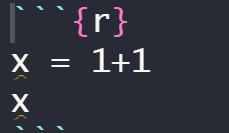
\includegraphics[width=0.15\linewidth]{Imgs/chunk_00}

que resulta en

\begin{Shaded}
\begin{Highlighting}[]
\NormalTok{x }\OtherTok{=} \DecValTok{1}\SpecialCharTok{+}\DecValTok{1}
\NormalTok{x}
\end{Highlighting}
\end{Shaded}

\begin{verbatim}
[1] 2
\end{verbatim}
\end{frame}

\begin{frame}{Chunks de R}
\protect\hypertarget{chunks-de-r-1}{}
Hay diversas opciones de crear un bloque de código de R:

\begin{itemize}
\tightlist
\item
  Ir al menú desplegable de ``Chunks'' y seleccionar el de R
\item
  Introducir manualmente
\item
  Alt + Command + I (para Mac) o Alt + Control + I (para Windows)
\end{itemize}
\end{frame}

\begin{frame}{Chunks de R}
\protect\hypertarget{chunks-de-r-2}{}
A los chunks se les puede poner etiqueta, para así localizarlos de
manera más fácil. Por ejemplo

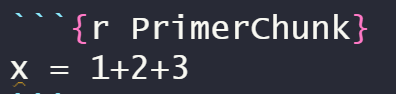
\includegraphics[width=0.6\linewidth]{Imgs/primer_chunk}

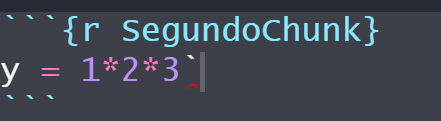
\includegraphics[width=0.6\linewidth]{Imgs/segundo_chunk}
\end{frame}

\begin{frame}[fragile]{Parámetros de los chunks}
\protect\hypertarget{paruxe1metros-de-los-chunks}{}
La parte entre llaves también puede contener diversos parámetros,
separados por comas entre ellos y separados de la etiqueta (o de r, si
hemos decidido no poner ninguna).

Estos parámetros determinan el comportamiento del bloque al compilar el
documento pulsando el botón \texttt{Knit} situado en la barra superior
del área de trabajo.
\end{frame}

\begin{frame}[fragile]{Parámetros de los chunks}
\protect\hypertarget{paruxe1metros-de-los-chunks-1}{}
\begin{longtable}[]{@{}
  >{\raggedright\arraybackslash}p{(\columnwidth - 2\tabcolsep) * \real{0.5000}}
  >{\raggedright\arraybackslash}p{(\columnwidth - 2\tabcolsep) * \real{0.5000}}@{}}
\toprule()
\begin{minipage}[b]{\linewidth}\raggedright
Código
\end{minipage} & \begin{minipage}[b]{\linewidth}\raggedright
Significado
\end{minipage} \\
\midrule()
\endhead
\texttt{echo} & Si lo igualamos a \texttt{TRUE}, que es el valor por
defecto, estaremos diciendo que queremos que se muestre el código fuente
del chunk. En cambio, igualado a \texttt{FALSE}, no se mostrará \\
\texttt{eval} & Si lo igualamos a \texttt{TRUE}, que es el valor por
defecto, estaremos diciendo que queremos que se evalúe el código. En
cambio, igualado a \texttt{FALSE}, no se evaluará \\
\bottomrule()
\end{longtable}
\end{frame}

\begin{frame}[fragile]{Parámetros de los chunks}
\protect\hypertarget{paruxe1metros-de-los-chunks-2}{}
\begin{longtable}[]{@{}
  >{\raggedright\arraybackslash}p{(\columnwidth - 2\tabcolsep) * \real{0.5000}}
  >{\raggedright\arraybackslash}p{(\columnwidth - 2\tabcolsep) * \real{0.5000}}@{}}
\toprule()
\begin{minipage}[b]{\linewidth}\raggedright
Código
\end{minipage} & \begin{minipage}[b]{\linewidth}\raggedright
Significado
\end{minipage} \\
\midrule()
\endhead
\texttt{message} & Nos permite indicar si queremos que se muestren los
mensajes que R produce al ejecutar código. Igualado a \texttt{TRUE} se
muestran, igualado a \texttt{FALSE} no \\
\texttt{warning} & Nos permite indicar si queremos que se muestren los
mensajes de advertencia que producen algunas funciones al ejecutarse.
Igualado a \texttt{TRUE} se muestran, igualado a \texttt{FALSE} no \\
\bottomrule()
\end{longtable}
\end{frame}

\begin{frame}[fragile]{Parámetros de los chunks}
\protect\hypertarget{paruxe1metros-de-los-chunks-3}{}
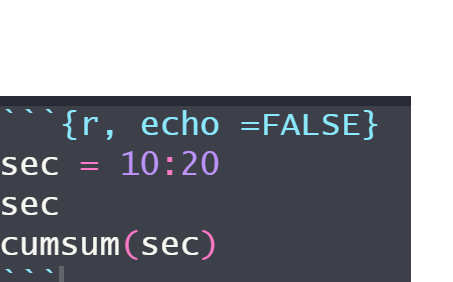
\includegraphics[width=0.5\linewidth]{Imgs/no_aparece}

No aparece el código solo la salida

\begin{verbatim}
 [1] 10 11 12 13 14 15 16 17 18 19 20
\end{verbatim}

\begin{verbatim}
 [1]  10  21  33  46  60  75  91 108 126 145 165
\end{verbatim}
\end{frame}

\begin{frame}[fragile]{Parámetros de los chunks}
\protect\hypertarget{paruxe1metros-de-los-chunks-4}{}
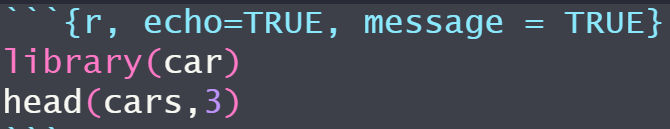
\includegraphics[width=0.6\linewidth]{Imgs/parametros_chunk_2}

\begin{Shaded}
\begin{Highlighting}[]
\FunctionTok{library}\NormalTok{(car)}
\end{Highlighting}
\end{Shaded}

\begin{verbatim}
Loading required package: carData
\end{verbatim}

\begin{Shaded}
\begin{Highlighting}[]
\FunctionTok{head}\NormalTok{(cars,}\DecValTok{3}\NormalTok{)}
\end{Highlighting}
\end{Shaded}

\begin{verbatim}
  speed dist
1     4    2
2     4   10
3     7    4
\end{verbatim}
\end{frame}

\begin{frame}[fragile]{Parámetros de los chunks}
\protect\hypertarget{paruxe1metros-de-los-chunks-5}{}
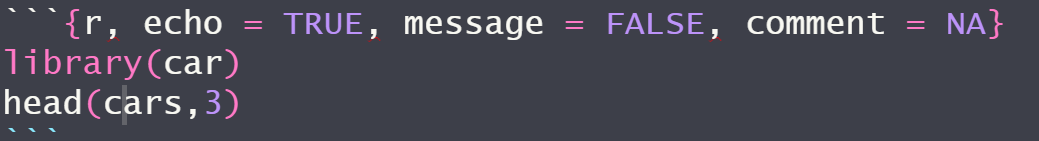
\includegraphics[width=0.6\linewidth]{Imgs/para_chunks_3}

\begin{Shaded}
\begin{Highlighting}[]
\FunctionTok{library}\NormalTok{(car)}
\FunctionTok{head}\NormalTok{(cars,}\DecValTok{3}\NormalTok{)}
\end{Highlighting}
\end{Shaded}

\begin{verbatim}
  speed dist
1     4    2
2     4   10
3     7    4
\end{verbatim}

Fijaos que \texttt{comment=NA} evita que aparezcan los \texttt{\#\#}
\end{frame}

\begin{frame}[fragile]{Parámetros de los chunks}
\protect\hypertarget{paruxe1metros-de-los-chunks-6}{}
\begin{longtable}[]{@{}
  >{\raggedright\arraybackslash}p{(\columnwidth - 4\tabcolsep) * \real{0.3333}}
  >{\raggedright\arraybackslash}p{(\columnwidth - 4\tabcolsep) * \real{0.3333}}
  >{\raggedright\arraybackslash}p{(\columnwidth - 4\tabcolsep) * \real{0.3333}}@{}}
\toprule()
\begin{minipage}[b]{\linewidth}\raggedright
Significado
\end{minipage} & \begin{minipage}[b]{\linewidth}\raggedright
Código
\end{minipage} & \begin{minipage}[b]{\linewidth}\raggedright
Resultado
\end{minipage} \\
\midrule()
\endhead
\texttt{results} & \texttt{markup} & Valor por defecto. Nos muestra los
resultados en el documento final línea a línea, encabezados por
\texttt{\#\#} \\
\texttt{results} & \texttt{hide} & No se nos muestra el resultado en el
documento final \\
\texttt{results} & \texttt{asis} & Nos devuelve los resultados línea a
línea de manera literal en el documento final y el programa con el que
se abre el documento final los interpreta como texto y formatea
adecuadamente \\
\texttt{results} & \texttt{hold} & Miestra todos los resultados al final
del bloque de código \\
\bottomrule()
\end{longtable}
\end{frame}

\begin{frame}[fragile]{Parámetros de los chunks}
\protect\hypertarget{paruxe1metros-de-los-chunks-7}{}
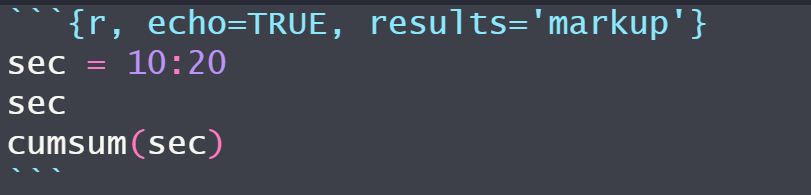
\includegraphics[width=0.6\linewidth]{Imgs/para_chunks_03}

\begin{Shaded}
\begin{Highlighting}[]
\NormalTok{sec }\OtherTok{=} \DecValTok{10}\SpecialCharTok{:}\DecValTok{20}
\NormalTok{sec}
\end{Highlighting}
\end{Shaded}

\begin{verbatim}
 [1] 10 11 12 13 14 15 16 17 18 19 20
\end{verbatim}

\begin{Shaded}
\begin{Highlighting}[]
\FunctionTok{cumsum}\NormalTok{(sec)}
\end{Highlighting}
\end{Shaded}

\begin{verbatim}
 [1]  10  21  33  46  60  75  91 108 126 145 165
\end{verbatim}
\end{frame}

\begin{frame}[fragile]{Parámetros de los chunks}
\protect\hypertarget{paruxe1metros-de-los-chunks-8}{}
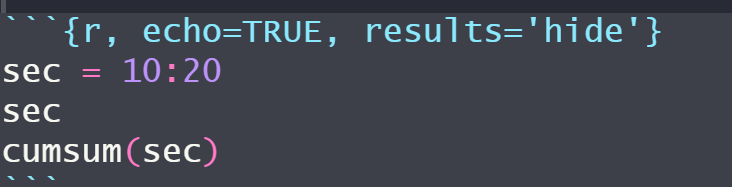
\includegraphics[width=0.6\linewidth]{Imgs/parametros_chunk_4}

\begin{Shaded}
\begin{Highlighting}[]
\NormalTok{sec }\OtherTok{=} \DecValTok{10}\SpecialCharTok{:}\DecValTok{20}
\NormalTok{sec}
\FunctionTok{cumsum}\NormalTok{(sec)}
\end{Highlighting}
\end{Shaded}
\end{frame}

\begin{frame}[fragile]{Parámetros de los chunks}
\protect\hypertarget{paruxe1metros-de-los-chunks-9}{}
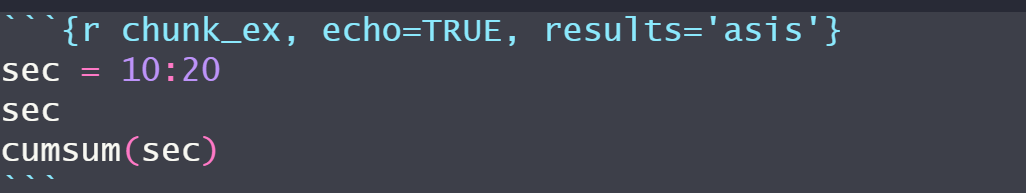
\includegraphics[width=0.6\linewidth]{Imgs/parametros_chunk_5}

\begin{Shaded}
\begin{Highlighting}[]
\NormalTok{sec }\OtherTok{=} \DecValTok{10}\SpecialCharTok{:}\DecValTok{20}
\NormalTok{sec}
\end{Highlighting}
\end{Shaded}

{[}1{]} 10 11 12 13 14 15 16 17 18 19 20

\begin{Shaded}
\begin{Highlighting}[]
\FunctionTok{cumsum}\NormalTok{(sec)}
\end{Highlighting}
\end{Shaded}

{[}1{]} 10 21 33 46 60 75 91 108 126 145 165
\end{frame}

\begin{frame}[fragile]{Parámetros de los chunks}
\protect\hypertarget{paruxe1metros-de-los-chunks-10}{}
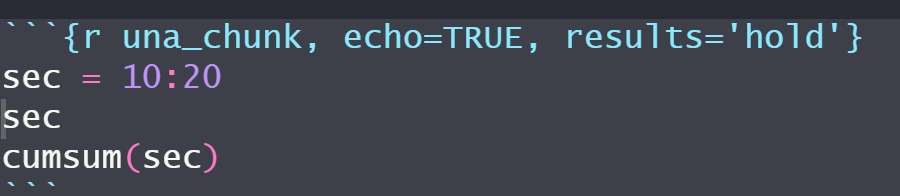
\includegraphics[width=0.6\linewidth]{Imgs/parametros_chunk_6}

\begin{Shaded}
\begin{Highlighting}[]
\NormalTok{sec }\OtherTok{=} \DecValTok{10}\SpecialCharTok{:}\DecValTok{20}
\NormalTok{sec}
\FunctionTok{cumsum}\NormalTok{(sec)}
\end{Highlighting}
\end{Shaded}

\begin{verbatim}
 [1] 10 11 12 13 14 15 16 17 18 19 20
 [1]  10  21  33  46  60  75  91 108 126 145 165
\end{verbatim}
\end{frame}

\hypertarget{estructuras-de-datos}{%
\section{Estructuras de datos}\label{estructuras-de-datos}}

\begin{frame}[fragile]{Tipos de datos en R, vectores}
\protect\hypertarget{tipos-de-datos-en-r-vectores}{}
Un \textbf{vector} es una secuencia ordenada de datos. \texttt{R}
dispone de muchos tipos de datos, por ejemplo:

\begin{itemize}
\tightlist
\item
  \texttt{logical}: lógicos (\texttt{TRUE} o \texttt{FALSE})
\item
  \texttt{integer}: números enteros, \(\mathbb Z\)
\item
  \texttt{numeric}: números reales, \(\mathbb R\)
\item
  \texttt{complex}: números complejos, \(\mathbb C\)
\item
  \texttt{character}: palabras
\end{itemize}

En los vectores de \texttt{R}, todos sus objetos han de ser del mismo
tipo: todos números, todos palabras, etc. Cuando queramos usar vectores
formados por objetos de diferentes tipos, tendremos que usar
\textbf{listas generalizadas}, \texttt{lists} que veremos al final del
tema.
\end{frame}

\begin{frame}[fragile]{Básico}
\protect\hypertarget{buxe1sico}{}
\begin{itemize}
\tightlist
\item
  \texttt{c()}: para definir un vector
\item
  \texttt{scan()}: para definir un vector
\item
  \texttt{fix(x)}: para modificar visualmente el vector \(x\)
\item
  \texttt{rep(a,n)}: para definir un vector constante que contiene el
  dato \(a\) repetido \(n\) veces
\end{itemize}

\begin{Shaded}
\begin{Highlighting}[]
\FunctionTok{c}\NormalTok{(}\DecValTok{1}\NormalTok{,}\DecValTok{2}\NormalTok{,}\DecValTok{3}\NormalTok{)}
\end{Highlighting}
\end{Shaded}

\begin{verbatim}
[1] 1 2 3
\end{verbatim}

\begin{Shaded}
\begin{Highlighting}[]
\FunctionTok{rep}\NormalTok{(}\StringTok{"Mates"}\NormalTok{,}\DecValTok{7}\NormalTok{)}
\end{Highlighting}
\end{Shaded}

\begin{verbatim}
[1] "Mates" "Mates" "Mates" "Mates" "Mates" "Mates" "Mates"
\end{verbatim}
\end{frame}

\begin{frame}{Función scan()}
\protect\hypertarget{funciuxf3n-scan}{}
\textbf{Ejemplo}

Vamos a crear un vector que contenga 3 copias de 1 9 9 8 0 7 2 6 con la
función scan:

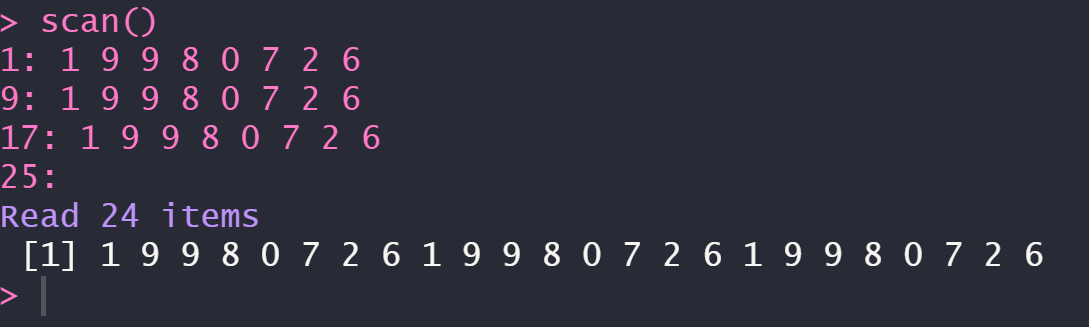
\includegraphics[width=0.6\linewidth]{Imgs/scan}
\end{frame}

\begin{frame}{Básico}
\protect\hypertarget{buxe1sico-1}{}
\textbf{Ejercicio}

\begin{enumerate}
\item
  Repite tu año de nacimiento 10 veces
\item
  Crea el vector que tenga como entradas
  \(16, 0, 1, 20, 1, 7, 88, 5, 1, 9\), llámalo vec y modifica la cuarta
  entrada con la función fix()
\end{enumerate}
\end{frame}

\begin{frame}[fragile]{Progresiones y Secuencias}
\protect\hypertarget{progresiones-y-secuencias}{}
Una progresión aritmética es una sucesión de números tales que la
\textbf{diferencia}, \(d\), de cualquier par de términos sucesivos de la
secuencia es constante. \[a_n = a_1 + (n-1)\cdot d\]

\begin{itemize}
\tightlist
\item
  \texttt{seq(a,b,by=d)}: para generar una
  \href{https://es.wikipedia.org/wiki/Progresión_aritmética}{progresión
  aritmética} de diferencia \(d\) que empieza en \(a\) hasta llegar a
  \(b\)
\item
  \texttt{seq(a,b,\ length.out=n)}: define progresión aritmética de
  longitud \(n\) que va de \(a\) a \(b\) con diferencia \(d\). Por tanto
  \(d=(b-a)/(n-1)\)
\item
  \texttt{seq(a,by=d,\ length.out=n)}: define la progresión aritmética
  de longitud \(n\) y diferencia \(d\) que empieza en \(a\)
\item
  \texttt{a:b}: define la secuencia de números \textbf{enteros}
  (\(\mathbb{Z}\)) consecutivos entre dos números \(a\) y \(b\)
\end{itemize}
\end{frame}

\begin{frame}{Secuencias}
\protect\hypertarget{secuencias}{}
\textbf{Ejercicio}

\begin{itemize}
\item
  Imprimid los números del 1 al 20
\item
  Imprimid los 20 primeros números pares
\item
  Imprimid 30 números equidistantes entre el 17 y el 98, mostrando solo
  4 cifras significativas
\end{itemize}
\end{frame}

\begin{frame}[fragile]{Funciones}
\protect\hypertarget{funciones}{}
Cuando queremos aplicar una función a cada uno de los elementos de un
vector de datos, la función \texttt{sapply} nos ahorra tener que
programar con bucles en \texttt{R}:

\begin{itemize}
\tightlist
\item
  \texttt{sapply(nombre\_de\_vector,FUN=nombre\_de\_función)}: para
  aplicar dicha función a todos los elementos del vector
\item
  \texttt{sqrt(x)}: calcula un nuevo vector con las raíces cuadradas de
  cada uno de los elementos del vector \(x\)
\end{itemize}
\end{frame}

\begin{frame}[fragile]{Funciones}
\protect\hypertarget{funciones-1}{}
Dado un vector de datos \(x\) podemos calcular muchas medidas
estadísticas acerca del mismo:

\begin{itemize}
\tightlist
\item
  \texttt{length(x)}: calcula la longitud del vector \(x\)
\item
  \texttt{max(x)}: calcula el máximo del vector \(x\)
\item
  \texttt{min(x)}: calcula el mínimo del vector \(x\)
\item
  \texttt{sum(x)}: calcula la suma de las entradas del vector \(x\)
\item
  \texttt{prod(x)}: calcula el producto de las entradas del vector \(x\)
\end{itemize}
\end{frame}

\begin{frame}[fragile]{Funciones}
\protect\hypertarget{funciones-2}{}
\begin{itemize}
\tightlist
\item
  \texttt{mean(x)}: calcula la media aritmética de las entradas del
  vector \(x\)
\item
  \texttt{diff(x)}: calcula el vector formado por las diferencias
  sucesivas entre entradas del vector original \(x\)
\item
  \texttt{cumsum(x)}: calcula el vector formado por las sumas acumuladas
  de las entradas del vector original \(x\)

  \begin{itemize}
  \tightlist
  \item
    Permite definir sucesiones descritas mediante sumatorios
  \item
    Cada entrada de \texttt{cumsum(x)} es la suma de las entradas de
    \(x\) hasta su posición
  \end{itemize}
\end{itemize}
\end{frame}

\begin{frame}[fragile]{Funciones}
\protect\hypertarget{funciones-3}{}
\begin{Shaded}
\begin{Highlighting}[]
\NormalTok{cuadrado }\OtherTok{=} \ControlFlowTok{function}\NormalTok{(x)\{x}\SpecialCharTok{\^{}}\DecValTok{2}\NormalTok{\}}
\NormalTok{v }\OtherTok{=} \FunctionTok{c}\NormalTok{(}\DecValTok{1}\NormalTok{,}\DecValTok{2}\NormalTok{,}\DecValTok{3}\NormalTok{,}\DecValTok{4}\NormalTok{,}\DecValTok{5}\NormalTok{,}\DecValTok{6}\NormalTok{)}
\FunctionTok{sapply}\NormalTok{(v, }\AttributeTok{FUN =}\NormalTok{ cuadrado)}
\end{Highlighting}
\end{Shaded}

\begin{verbatim}
[1]  1  4  9 16 25 36
\end{verbatim}

\begin{Shaded}
\begin{Highlighting}[]
\FunctionTok{mean}\NormalTok{(v)}
\end{Highlighting}
\end{Shaded}

\begin{verbatim}
[1] 3.5
\end{verbatim}

\begin{Shaded}
\begin{Highlighting}[]
\FunctionTok{cumsum}\NormalTok{(v)}
\end{Highlighting}
\end{Shaded}

\begin{verbatim}
[1]  1  3  6 10 15 21
\end{verbatim}
\end{frame}

\begin{frame}[fragile]{Orden}
\protect\hypertarget{orden}{}
\begin{itemize}
\tightlist
\item
  \texttt{sort(x)}: ordena el vector en orden natural de los objetos que
  lo forman: el orden numérico creciente, orden alfabético\ldots{}
\item
  \texttt{rev(x)}: invierte el orden de los elementos del vector \(x\)
\end{itemize}

\begin{Shaded}
\begin{Highlighting}[]
\NormalTok{v }\OtherTok{=} \FunctionTok{c}\NormalTok{(}\DecValTok{1}\NormalTok{,}\DecValTok{7}\NormalTok{,}\DecValTok{5}\NormalTok{,}\DecValTok{2}\NormalTok{,}\DecValTok{4}\NormalTok{,}\DecValTok{6}\NormalTok{,}\DecValTok{3}\NormalTok{)}
\FunctionTok{sort}\NormalTok{(v)}
\end{Highlighting}
\end{Shaded}

\begin{verbatim}
[1] 1 2 3 4 5 6 7
\end{verbatim}

\begin{Shaded}
\begin{Highlighting}[]
\FunctionTok{rev}\NormalTok{(v)}
\end{Highlighting}
\end{Shaded}

\begin{verbatim}
[1] 3 6 4 2 5 7 1
\end{verbatim}
\end{frame}

\begin{frame}[fragile]{Orden}
\protect\hypertarget{orden-1}{}
\textbf{Ejercicio}

\begin{itemize}
\item
  Combinad las dos funciones anteriores, \texttt{sort} y \texttt{rev}
  para crear una función que dado un vector \(x\) os lo devuelva
  ordenado en orden decreciente.
\item
  Razonad si aplicar primero \texttt{sort} y luego \texttt{rev} a un
  vector \(x\) daría en general el mismo resultado que aplicar primero
  \texttt{rev} y luego \texttt{sort}.
\item
  Investigad la documentación de la función \texttt{sort} (recordad que
  podéis usar la sintaxis \texttt{?sort} en la consola) para leer si
  cambiando algún argumento de la misma podéis obtener el mismo
  resultado que habéis programado en el primer ejercicio.
\end{itemize}
\end{frame}

\begin{frame}[fragile]{Subvectores}
\protect\hypertarget{subvectores}{}
\begin{itemize}
\item
  \texttt{vector{[}i{]}}: da la \(i\)-ésima entrada del vector

  \begin{itemize}
  \tightlist
  \item
    Los índices en R empiezan en 1
  \item
    \texttt{vector{[}length(vector){]}}: nos da la última entrada del
    vector
  \item
    \texttt{vector{[}a:b{]}}: si \(a\) y \(b\) son dos números
    naturales, nos da el subvector con las entradas del vector original
    que van de la posición \(a\)-ésima hasta la \(b\)-ésima.
  \item
    \texttt{vector{[}-i{]}}: si \(i\) es un número, este subvector está
    formado por todas las entradas del vector original menos la entrada
    \(i\)-ésima. Si \(i\) resulta ser un vector, entonces es un vector
    de índices y crea un nuevo vector con las entradas del vector
    original,cuyos índices pertenecen a \(i\)
  \item
    \texttt{vector{[}-x{]}}: si \(x\) es un vector (de índices),
    entonces este es el complementario de vector{[}\(x\){]}
  \end{itemize}
\end{itemize}
\end{frame}

\begin{frame}[fragile]{Subvectores}
\protect\hypertarget{subvectores-1}{}
\begin{itemize}
\item
  También podemos utilizar operadores lógicos:

  \begin{itemize}
  \tightlist
  \item
    \texttt{==}: =
  \item
    \texttt{!=}: \(\neq\)
  \item
    \texttt{\textgreater{}=}: \(\ge\)\\
  \item
    \texttt{\textless{}=}: \(\le\)
  \item
    \texttt{\textless{}}: \(<\)
  \item
    \texttt{\textgreater{}}: \(>\)
  \item
    \texttt{!}: NO lógico
  \item
    \texttt{\&}: Y lógico
  \item
    \texttt{\textbar{}}: O lógico
  \end{itemize}
\end{itemize}
\end{frame}

\begin{frame}[fragile]{Subvectores}
\protect\hypertarget{subvectores-2}{}
\begin{Shaded}
\begin{Highlighting}[]
\NormalTok{v }\OtherTok{=} \FunctionTok{c}\NormalTok{(}\DecValTok{14}\NormalTok{,}\DecValTok{5}\NormalTok{,}\DecValTok{6}\NormalTok{,}\DecValTok{19}\NormalTok{,}\DecValTok{32}\NormalTok{,}\DecValTok{0}\NormalTok{,}\DecValTok{8}\NormalTok{)}
\NormalTok{v[}\DecValTok{2}\NormalTok{]}
\end{Highlighting}
\end{Shaded}

\begin{verbatim}
[1] 5
\end{verbatim}

\begin{Shaded}
\begin{Highlighting}[]
\NormalTok{v[}\SpecialCharTok{{-}}\FunctionTok{c}\NormalTok{(}\DecValTok{3}\NormalTok{,}\DecValTok{5}\NormalTok{)]}
\end{Highlighting}
\end{Shaded}

\begin{verbatim}
[1] 14  5 19  0  8
\end{verbatim}

\begin{Shaded}
\begin{Highlighting}[]
\NormalTok{v[v }\SpecialCharTok{!=} \DecValTok{19} \SpecialCharTok{\&}\NormalTok{ v}\SpecialCharTok{\textgreater{}}\DecValTok{15}\NormalTok{]}
\end{Highlighting}
\end{Shaded}

\begin{verbatim}
[1] 32
\end{verbatim}
\end{frame}

\begin{frame}[fragile]{Condicionales}
\protect\hypertarget{condicionales}{}
\begin{itemize}
\tightlist
\item
  \texttt{which(x\ cumple\ condición)}: para obtener los índices de las
  entradas del vector \(x\) que satisfacen la condición dada
\item
  \texttt{which.min(x)}: nos da la primera posición en la que el vector
  \(x\) toma su valor mínimo
\item
  \texttt{which(x==min(x))}: da todas las posiciones en las que el
  vector \(x\) toma sus valores mínimos
\item
  \texttt{which.max(x)}: nos da la primera posición en la que el vector
  \(x\) toma su valor máximo
\item
  \texttt{which(x==max(x))}: da todas las posiciones en las que el
  vector \(x\) toma sus valores máximos
\end{itemize}
\end{frame}

\end{document}
